% gm-final-exam-mock.tex

\documentclass[11pt]{article}
\usepackage{enumerate}
\usepackage{syllogism} 
\usepackage{october}
\usepackage[table]{xcolor}

% testing overleaf

\begin{document}

\textbf{Mock Final Exam}

The final exam will NOT look like this. The final exam is a selection
of questions with more emphasis on material covered later in the
course. This list contains one question for each category so that you
can check what you are good at and what you need to practice more. The
solutions are posted online.

\begin{enumerate}
\item Solve the following system of linear equations.
  \begin{equation}
    \label{eq:oedeoyai}
    \begin{array}{lclcr}
      0.3x & + & 0.2y & = & -0.9 \\
      0.2x & - & 0.3y & = & -0.6
    \end{array}
  \end{equation}
\item Two planes travel toward each other from cities that are 780 km
  apart at speeds of 190 and 200 km/h. They started at the same time.
  In how many hours will they meet?
\item Solve the following quadratic equation.
  \begin{equation}
    \label{eq:eishahji}
    6y^{2}-2\sqrt{3}y-1=0
  \end{equation}
\item Solve the following exponential equation.
  \begin{equation}
    \label{eq:vohtovuj}
    25^{3x-2}=625^{2x+7}
  \end{equation}
\item Solve the following logarithmic equation.
  \begin{equation}
    \label{eq:laishedu}
    \log_{8}(x+1)-\log_{8}x=\log_{8}4
  \end{equation}
\item Solve the following trigonometric equation in $\{x\in\mathbb{R}|0^{\circ}\leq{}x<360^{\circ}\}$
  \begin{equation}
    \label{eq:iegheovi}
    \sin{}2x\cos{}x-\sin{}x=0    
  \end{equation}
\item What are slope and $y$-intercept of the curve corresponding to
  the following linear equation?
  \begin{equation}
    \label{eq:eopifeek}
    3x+y=\pi
  \end{equation}
\item Three circles are arranged as in the figure below. Find the
  angle $\phi$. (The radius of the circles is $28,22,36$,
  respectively; the angle shown is $41^{\circ}$.)
    \begin{figure}[h]
    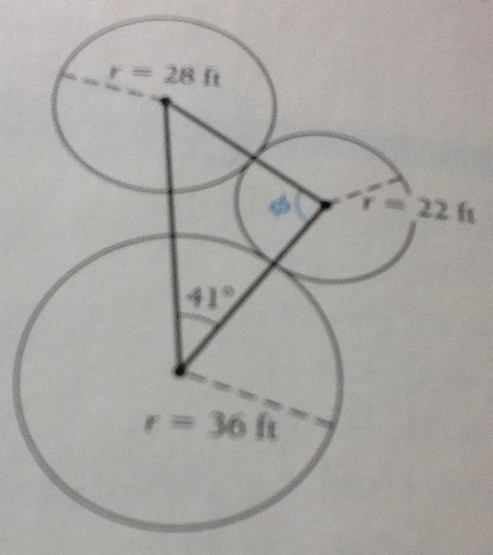
\includegraphics[scale=.5]{./threecircles.png}
  \end{figure}
\item Simplify the following expression.
  \begin{equation}
    \label{eq:oocohlie}
    \sqrt{2x^{2}-(x-5)(x+5)-10x}
  \end{equation}
\item Identify the centre and the dimensions of the box for the
  following hyperbola:
  \begin{equation}
    \label{eq:uzahpahp}
    \frac{1}{2}y^{2}+\frac{5}{2}=x^{2}+6x+5y
  \end{equation}
\item An airplane travels on a bearing of $100^{\circ}$ at a 180 km/h
  airspeed while a wind is blowing 45 km/h from 220$^{\circ}$. Find
  the speed of the airplane over the ground and the direction of its
  track over the ground.
  % Solution: Bittinger Beecher page 528
\item In professional tennis, there are about 600 challenges made to
  referee calls in single play during one year. 30\% of challenges are
  upheld with the call overturned, according to long years of
  experience. What approximately is the probability that this year
  between 175 and 200 challenges will be upheld, i.e.\ no fewer than
  175 and no more than 200?
\item Based on a large data set, you conclude that the amount of sleep
   that you get at night is normally distributed with a mean of $8.09$ hours
   and a standard deviation of $52$ minutes. What is the probability
   that you will get less than 7 hours of sleep tonight?
 \item Solve the following spherical triangles.
   \begin{equation}
     \label{eq:isotufie}
     a=67^{\circ}19'30''\;{}b=52^{\circ}18'20''\;{}c=37^{\circ}13'50''
     % Clifford Bell, page 151
   \end{equation}
   \begin{equation}
     \label{eq:eizokaih}
     b=21^{\circ}30'5''\;{}B=58^{\circ}10'15''\;{}C=90^{\circ}
     % Clifford Bell, page 131
   \end{equation}
\end{enumerate}

\end{document}

